%% IEEE TKDE (Transactions on Knowledge and Data Engineering) format
%% Build: latexmk -pdf main_tkde.tex
\documentclass[10pt,journal,compsoc]{IEEEtran}

\usepackage{graphicx}
\usepackage{amsmath}
\usepackage{amssymb}
\usepackage{booktabs}
\usepackage{array}
\usepackage{url}
\usepackage[nocompress]{cite}
\usepackage{enumitem}
\setlist{itemsep=1pt,topsep=3pt,parsep=0pt}
\newcolumntype{P}[1]{>{\raggedright\arraybackslash}p{#1}}
\emergencystretch=3em
\setlength{\textfloatsep}{8pt plus 2pt minus 3pt}\setlength{\floatsep}{6pt plus 2pt minus 2pt}\setlength{\dbltextfloatsep}{8pt plus 2pt minus 3pt}\setlength{\dblfloatsep}{6pt plus 2pt minus 2pt}
% Run-in paragraph headings: no numbering, and no second punctuation mark after the title's own period.
\setcounter{secnumdepth}{3}
\let\wrgOldParagraph\paragraph
\def\wrgStripDot#1.\relax{#1}
\renewcommand{\paragraph}[1]{\wrgOldParagraph{\wrgStripDot#1\relax}}

% Figures produced separately appear in figures/. The build passes before they exist.
\newcommand{\figseedref}{{, Fig.~\ref{fig:seedforest}}}
\newcommand{\figcostref}{{, Fig.~\ref{fig:costquality}}}

\newcommand{\releaseurl}{Code, plans and graphs: [anonymized].}
\renewcommand{\arraystretch}{0.9}
\begin{document}

\title{What Reaches the Graph Decides Held-Out Question Answering in Knowledge Graph Construction}

\author{Anonymous Authors}

% The paper headers
\markboth{IEEE Transactions on Knowledge and Data Engineering,~Vol.~XX, No.~X, Month~2026}%
{Anonymous Authors: What Reaches the Graph Decides Held-Out Question Answering}

\IEEEtitleabstractindextext{%
\begin{abstract}
LLM knowledge-graph pipelines generate competency questions (CQs) from text, derive a schema and repair the graph where CQs fail. We remove each step in turn with Qwen on 2WikiMultihopQA (2Wiki), T-REx and HotpotQA, scoring graphs on unseen questions. In our rebuilt CQ pipelines on 2Wiki, the gain comes from a flat list of 22 relation names, not from the CQs or the repair loop: the list raises grounded QA (answers supported by retrieved facts) in all four pipelines, by 4.5 to 14.7 points. One extraction pass given only the list (the list-schema pass) leads our full list-plus-CQ pipeline in grounded QA when the answerer sees up to 60 facts, by 4.6 points with the gold-derived list and 5.3 with a corpus-induced one, and is level with it in answer correctness at one eighth of the tokens. Deriving the schema from generated CQs instead costs 11.1 points. Seeded extraction, with the list in every chunk's prompt, is 6.7 to 8.3 times cheaper than the repair loop on 2Wiki but stores facts under hundreds of relation names, passing 7.5\% of SPARQL tests against 34.9\% for the list-schema pass. On HotpotQA, whose relations are long-tailed, an induced list lowers plain extraction by 4.0.
\end{abstract}


\begin{IEEEkeywords}
Competency questions, knowledge graph construction, large language models, question answering, relation list.
\end{IEEEkeywords}}

\maketitle

\IEEEdisplaynontitleabstractindextext
\IEEEpeerreviewmaketitle

\section{Introduction}
\label{sec:intro}

Nothing guarantees that a graph a large language model (LLM) pipeline builds from text can answer the questions people will ask. Ontology engineering approaches this with competency questions~\cite{gruninger1995methodology,noy2001ontology101}. Here a competency question (CQ) is a test question generated from a text chunk, with an expected answer span. Recent pipelines generate CQs from text, grow a schema from them and repair what fails. We call this cycle the repair loop: build the graph, write test questions, find the ones it cannot answer, and patch the graph, repeatedly (Section~\ref{sec:pipeline}).

Consider the question ``What is the cause of death of director of film Wedding Bills?'' from 2WikiMultihopQA (2Wiki)~\cite{ho2020twowiki}, multi-hop questions over Wikipedia. The source text says the director died ``from Parkinson's disease''. With Qwen, an open-weight LLM family, the graph built by the CQ-guided single pass (one extraction pass whose schema comes from 40 generated CQs) with no relation list has no cause-of-death triple for him, and the answerer says ``unknown''. Given a relation list, here 22 relation names that include ``cause of death'', the same pipeline extracts the triple and answers correctly. The relation list is a flat vocabulary of names, with no types or ranges, and is the variable this paper isolates.

Published CQ-driven pipelines~\cite{feng2024ontologygrounded,kaiser2025hydra,choi2026socratickg} and loops~\cite{huang2025tcrqf,chong2026evoontology,zhang2026oak} change several components at once and report one final score, which cannot say where a gain comes from. We rebuild their components in one pipeline family rather than rerun each system. This study scores finished graphs on held-out questions and tests the repair step against random patches of the same size.

We build a graph from text, then test it with questions it never saw. A fact helps held-out question answering (QA) only if the graph contains it and retrieval returns it: removing the gold-evidence facts from what the answerer sees lowers answer correctness by 40 points or more (Appendix~\ref{app:reach}). Our main measure, grounded QA, is the share of held-out questions answered correctly from retrieved graph facts that contain the answer, scored by code; answer correctness drops the support requirement, and the SPARQL pass rate measures querying the graph. The answerer sees at most 60 retrieved facts (the answer fact cap). The corpora are 2Wiki, a T-REx~\cite{elsahar2018trex} movie subset with one-hop questions, and HotpotQA~\cite{yang2018hotpotqa}. Values are means over shards (groups of questions with their source paragraphs; a unit is one shard built under one run seed), and differences are in points with 95\% intervals over shards; two arms are \emph{level} when that interval includes zero.

An arm is a pipeline variant, and the relation list is the variable that separates them. We compare these arms (Table~\ref{tab:arms} gives the full definitions):
\begin{itemize}[nosep]
  \item \emph{CQ-guided single pass}: one extraction pass whose schema comes from 40 generated CQs.
  \item \emph{Repair loop}: the CQ-guided single pass plus rounds of new CQs that test and patch the graph.
  \item \emph{Plain extraction}: every chunk extracted with free-form predicates, no CQs, no list.
  \item \emph{Seeded extraction}: plain extraction with the relation list in every prompt; predicates stay free-form.
  \item \emph{List-schema pass}: one pass whose schema is only the 22 list names, no CQs; predicates are restricted to those names.
  \item \emph{Combined pipeline} (our full list-plus-CQ pipeline): the list, CQs for every chunk, extra extraction passes, CQ evaluation.
\end{itemize}
Our main result is that on 2Wiki the relation list, not the chunk-generated CQs or the repair loop, produces the held-out QA gain. Three findings follow.

(1) On 2Wiki, a list-schema pass matches the combined pipeline built with the same list in answer correctness at one eighth of its construction tokens, and leads it in grounded QA when the answerer sees up to 60 facts: by 4.6 points with the 22 most frequent gold relation types and by 5.3 with a list induced without gold (60 units each). At 120 facts, where no cap binds, the two are level. A single pass whose schema comes from generated CQs, given the same list, scores 11.1 points lower; CQs pay off on the questions their own generator writes, where the combined pipeline leads by 18.1 points.

(2) Seeded extraction costs 6.7 to 8.3 times fewer tokens than the repair loop on 2Wiki, 7.1 on HotpotQA and 16 to 17 on T-REx, but it stores its facts under hundreds of relation names and passes only 7.5\% of the SPARQL tests; mapping its predicates to the 22 list names recovers about half of the lost SPARQL passes.

(3) The repair loop's lead depends on question type and corpus: pooled over 60 2Wiki shards it leads seeded extraction by 3.2 points in grounded QA, all of it from bridge-comparison questions (it trails on comparison questions); on HotpotQA seeded extraction leads at every fact cap, and an induced list lowers plain extraction by 4.0 points ($+$0.8 on 2Wiki).

We release plans, deviation logs, code and graphs.\footnote{\releaseurl}

\section{Related Work}
\label{sec:related}

\paragraph{Competency questions and LLM-assisted ontology engineering.}
Competency questions fix the scope of an ontology before it is built~\cite{gruninger1995methodology,noy2001ontology101}. Feng et al.\ derive relations from CQs and ground graph construction in the resulting ontology~\cite{feng2024ontologygrounded}. HyDRA builds an ontology from CQs that agents agree on~\cite{kaiser2025hydra}, and SocraticKG expands each passage into question--answer pairs before extraction~\cite{choi2026socratickg}. Other work assists CQ writing~\cite{zhang2024ontochat,pan2024rag}, pairs CQs with SPARQL~\cite{taghzouti2025q2forge} or builds ontologies with LLMs~\cite{lippolis2025ontogenia}; these works judge the ontology or the CQs, and we judge the resulting graph on unseen questions.

Graph-based RAG systems build graphs for retrieval rather than for CQ-driven construction: GraphRAG combines an entity graph with community summaries~\cite{edge2024graphrag}, and HippoRAG retrieves over a passage graph with personalised PageRank~\cite{gutierrez2024hipporag}; whether a graph helps RAG at all depends on the task~\cite{xiang2026graphragbench}. Their indexing also extracts from every chunk~\cite{guo2024lightrag}; seeded extraction is that indexing step given a relation list, and we compare at the graph-construction stage and against HippoRAG 2 end to end (Section~\ref{sec:res-cost}).

\paragraph{Iterative repair.}
TCR-QF, EvoOntology and OaK repair a graph or an ontology over several rounds~\cite{huang2025tcrqf,chong2026evoontology,zhang2026oak}. None of these CQ pipelines or loops is compared with a baseline that keeps the relation list and drops the CQs, so their gains cannot be split between the list and the CQ machinery. This paper makes that split: it removes one component at a time, scores finished graphs on held-out questions, and tests the repair step against random patches of the same size.

\paragraph{Text-to-KG extraction, schema-guided extraction, schema induction and QA-based evaluation.}
iText2KG builds graphs incrementally without a fixed schema~\cite{lairgi2024itext2kg}, and Text2KGBench scores extraction when the ontology is given~\cite{mihindukulasooriya2023text2kgbench}. CodeKGC and KnowCoder encode a schema in code prompts~\cite{bi2024codekgc,li2024knowcoder}, and GoLLIE reports that label definitions in the schema are central to zero-shot extraction~\cite{sainz2024gollie}. EDC (Extract, Define, Canonicalize) runs with a pre-defined target schema or one it induces and canonicalises itself~\cite{zhang2024edc}, and AutoSchemaKG induces a schema from text and reports multi-hop QA gains~\cite{bai2026autoschemakg}, and KGGen clusters the entities and relations it extracts~\cite{mo2025kggen}. On our data the fixed list reached higher evidence recall than prompts tuned by MIPROv2 or GEPA~\cite{opsahlong2024mipro,agrawal2025gepa} (Appendix~\ref{app:promptopt}). These works score extraction under a schema; we ask which component of a CQ-driven pipeline produces its held-out QA gain.

\section{Pipeline and Experimental Design}
\label{sec:pipeline-design}
\subsection{The Curation Pipeline and Its Components}
\label{sec:pipeline}

All experiments use one pipeline family, which reads a corpus split into chunks and produces a schema and a set of facts stored as Resource Description Framework (RDF) triples. In the CQ pipelines the schema holds classes and properties derived from the CQs; in the list-schema pass it is only the relation list. Formally, a constructed knowledge graph is represented as $G = (V, E)$, where $V$ denotes the set of entity vertices and $E \subseteq V \times \mathcal{R} \times V$ denotes directed relational edges labeled by predicates from a relation vocabulary $\mathcal{R}$. Figure~\ref{fig:pipeline} shows the five stages, and Appendix Table~\ref{tab:experiments} lists the eight studies.

\begin{figure*}[t]
\centering
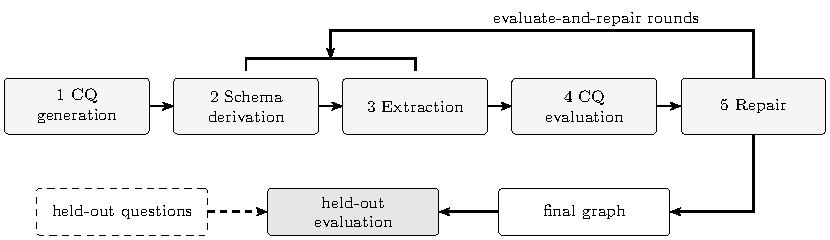
\includegraphics[width=0.74\textwidth]{fig_pipeline.pdf}
\caption{The pipeline builds the graph in five stages, and evaluate-and-repair rounds loop from repair back to schema derivation and extraction. Held-out questions reach only the evaluation of the final graph.}
\label{fig:pipeline}
\end{figure*}

\paragraph{Stages.}
\begin{enumerate}
  \item \emph{CQ generation.} The generator reads a batch of chunks and writes questions that a reader of those chunks should be able to answer. Each CQ, a question generated from a chunk, keeps its source chunk and an expected answer span, which code checks against the chunk.
  \item \emph{Schema derivation.} Classes and properties are derived from the CQs.
  \item \emph{Extraction.} Facts are extracted chunk by chunk, guided by the current schema. Every fact keeps the chunk it came from.
  \item \emph{CQ evaluation.} Each CQ is translated to SPARQL Protocol and RDF Query Language (SPARQL) queries and run against the graph. A deterministic rule first checks that the expected span appears in the result rows. An LLM judge then grades the answer 0, 1 or 2.
  \item \emph{Repair.} Failed CQs are attributed either to the query or to the graph. Graph-side failures produce patches (added facts, merged entities, corrected values or new properties). A gate scores each patch on a reserved set of curation CQs, never on held-out questions, and accepts or rejects it.
\end{enumerate}

\paragraph{Components under test.}
Every study except the error analysis changes one of the following components or removes one from the combined pipeline.
\begin{description}
  \item[Relation list.] A relation list from the training split: the 22 most frequent relation types (share of at least 0.1\%) among the gold evidence relations annotated in the 2WikiMultihopQA training split, where no evaluation question was used. The names cover the relations of 98.4\% of the 1,216 gold evidence items. The prompts receive the names only, without types, domains or ranges, as one block with the same wording and position in every arm with the list (Table~\ref{tab:arms}; names in Appendix~\ref{app:seednames}). Below, ``the list'' is this relation list.
  \item[CQ coverage.] Coverage is the share of chunks that are the source of at least one CQ. A first round writes a fixed number of CQs (40 in most experiments). \emph{Expansion} adds CQs over several rounds, each time drawing from chunks that are not yet the source of any CQ, until every chunk is covered.
  \item[CQ count.] One study varies the number of CQs at a fixed or increased token budget.
  \item[Evaluate-and-repair rounds.] Stages 4 and 5 run for several rounds. The loop repairs queries first and patches only graph-side failures.
  \item[Settings of the CQ arms.] Settings that could hold the CQ arms back are varied: 160 instead of 40 CQs at up to four times the budget (Appendix Table~\ref{tab:exp9}), CQs on every chunk plus extra passes (the combined pipeline), and the schema cut or restricted to the 22 names (Section~\ref{sec:res-schema}).
  \item[Budget and extraction passes.] The total number of tokens, and how the remainder is spent. In the combined pipeline, tokens left after expansion go to additional full-corpus extraction passes that ask for facts missing from the current graph.
\end{description}

\paragraph{Induced lists.}
An \emph{induced list} uses no question and no gold relation. The extraction model proposes relation names from 300 randomly sampled passages, and one model call merges the most frequent proposals into exactly 22 names, so induced lists equal the original list in size and differ only in content (Appendices~\ref{app:seednames} and~\ref{app:registration}).

Table~\ref{tab:arms} defines every arm; the text uses plain names and the tables the codes. The \emph{combined pipeline} (``Combined'') starts from the relation list, and a \emph{+vocab} suffix on any other arm code means the same pipeline run with that list.

\begin{table*}[t]
\centering
\small\setlength{\tabcolsep}{3.5pt}
\caption{The arms compared, as ``plain name in the text (code in tables)''. ``Reads and writes'' gives what each arm takes in and produces; the last column gives where the relation list, the 22 names given to the prompts, enters when the arm runs with it. The expansion arms (G, GR) and the $K$-name arms are in Appendix~\ref{app:armsextra}.}
\label{tab:arms}
\begin{tabular}{P{4.2cm}P{6.0cm}cP{4.2cm}}
\toprule
Arm & Reads and writes & CQs & Where the list enters \\
\midrule
CQ-guided single pass (L0) & Chunks $\rightarrow$ 40 CQs $\rightarrow$ schema ($\le$36 properties) $\rightarrow$ facts from every chunk & yes & CQ generation, schema derivation \\
Repair loop (LOOP) & L0, then 3 rounds of CQ evaluation and repair (20 new CQs per round) & yes & CQ generation, schema extension, schema patches \\
Combined pipeline (Combined) & Relation list; CQs expanded to every chunk; incremental schema with de-duplication; extra extraction passes (to about 95\% of LOOP+vocab's tokens); CQ evaluation as acceptance test, no repair & yes & CQ generation, schema derivation, schema extension \\
Plain extraction (U-ext) & No CQs, no schema: free-form predicates, one call per chunk; schema derived afterwards & no & none \\
Seeded extraction (U-ext+vocab) & U-ext run with the 22-name list & no & Extraction prompt, after the chunk text \\
+vocab & Any other arm run with the 22-name list (L0+vocab is the CQ-guided single pass with the list); Combined always has it unless marked no list & as arm & as in the arm's row \\
List-schema pass (S0) & No CQs: the 22 list names alone are the schema. The 22 list names $\rightarrow$ schema (22 properties) $\rightarrow$ facts from every chunk & no & Schema derivation \\
iText2KG, EDC, AutoSchemaKG & Chunks $\rightarrow$ facts, released settings, no list (EDC once with the list, Appendix Table~\ref{tab:itext}); EDC and AutoSchemaKG induce their own schema; AutoSchemaKG's entity-relation triples are scored & no & none \\
\bottomrule
\end{tabular}
\end{table*}

\subsection{Experimental Design}
\label{sec:design}

\paragraph{Data.}
Dataset questions are held out from every stage of construction and only score the final graph; an induced list reads corpus passages but no question.

The main corpus is 2WikiMultihopQA (2Wiki)~\cite{ho2020twowiki}. A \emph{shard} is a group of questions together with the union of their context paragraphs, and a \emph{unit} is one shard in one run seed (60 units = 30 shards $\times$ 2 run seeds). Shards hold about 16 questions (8 in the first patch study; Appendix Table~\ref{tab:experiments}), and each 2Wiki study after the first excludes the questions used in earlier ones; the main study holds 480 held-out questions.

The second corpus is a movie-domain subset of T-REx~\cite{elsahar2018trex} with 482 documents and 14 relation types, of which 386 documents and 507 questions are held out, in 33 shards. The T-REx arm of the 2Wiki main study (Appendix Table~\ref{tab:newchecks}, Fig.~\ref{fig:costquality}) used the 22 names of the 2Wiki list; Appendix~\ref{app:trexlist} used 22 names induced from T-REx. The third corpus is HotpotQA~\cite{yang2018hotpotqa} (distractor setting, crowd-written questions): 480 held-out questions in 30 shards, one run, and a 22-name list induced from 300 training paragraphs disjoint from the evaluation shards.

\paragraph{Metrics.}
We score a graph by held-out QA over the facts retrieved from it. Grounded QA counts a question when an answer written from graph facts alone is correct and the gold answer appears in a retrieved fact; answer correctness drops the grounding requirement. Both are scored by code, as are evidence recall (the share of gold evidence triples in the graph) and relation accuracy (the share of them with the right entity pair, relation and direction), the supporting measures. Hybrid QA lets the answerer see passages as well as graph facts; the SPARQL pass rate and hybrid QA are defined in Appendix~\ref{app:metricdefs}. Retrieval links question words to entities, expands two hops and ranks facts by BM25 (Appendices~\ref{app:groundedret} and~\ref{app:altret}). An LLM judge scores the pipeline's internal CQ evaluation and the SPARQL pass rates (the builder's family) and fact precision (the other family). Values are shard-weighted means; scoring details are in Appendix~\ref{app:details}.

\paragraph{Models.}
Construction, querying and QA use Qwen3.8-Flash-Next (checkpoint \texttt{Qwen/Qwen3.8-Flash-Next}, served with 4-bit NVFP4 weights) in all studies but the CQ-count study, which runs Qwen and Gemma on both corpora; the Gemma replication repeats the studies named in Appendix Table~\ref{tab:experiments} with Gemma-4-26B-A4B-it (\texttt{google/gemma-4-26B-A4B-it}).

\paragraph{Plans and statistics.}
Each experiment has a plan fixed before the main run (Appendix~\ref{app:registration}). The unit of analysis is the shard, and intervals are two-sided 95\% bootstrap intervals that resample shards.

Tokens per unit count an arm's construction and its own CQ evaluation (SPARQL and judge calls, which seeded extraction does not make), with retries counted, and exclude the held-out QA that scores the graph, which is of similar size across arms (16k to 23k per unit) under the same 60-fact cap (Appendix~\ref{app:details}). Inducing a list is a one-time cost per corpus (Appendix~\ref{app:induction}). The combined pipeline stopped at about 95\% of the loop's tokens with the list on the same unit (838k against 878k), and its arm without the list used the same budget.

The equal-fact-count check draws a uniform random subset of the facts in each stored graph of plain extraction, with and without the list, down to the fact count $|E|$ of the corresponding CQ-guided single-pass graph. Six selectors reduce the same graphs to the same fact count without reading questions or gold (Appendix~\ref{app:details} and Table~\ref{tab:selection}).

\section{The List, Not the CQs, Explains the Single Pass's Gain}
\label{sec:res-schema}

On the 60 main-run 2Wiki units the list-schema pass scores .652 grounded QA, 4.6 points above the combined pipeline (.606), at one eighth of its tokens (Section~\ref{sec:res-cost}). This section traces that gain to the list. Without the list, CQ guidance scores below plain extraction (.394 against .558 grounded QA, Table~\ref{tab:exp8}).
\paragraph{The list-schema pass, with no CQs, scores above the CQ-guided single pass given the same list.}
The list-schema pass makes one extraction pass whose schema is the 22 list names alone. On the 60 main-run units it scored 11.1 points above the CQ-guided single pass given the same list (.652 against .541; [7.5, 14.3]; answer correctness +11.8 [8.9, 14.8]). Schema size does not explain the gap. In a 30-unit factorial run (Appendix Table~\ref{tab:listschema}), cutting the CQ-derived schema to 22 properties moved grounded QA by +0.2 [$-$1.9, 2.9]; deriving it from the same CQs but restricted to the 22 names raised it by 7.3 [3.3, 12.1], and the 22 names alone, with no CQs, added 4.2 more [0.6, 7.3]. On T-REx it gains 4.4 points over the CQ-guided single pass; on HotpotQA it is level with it (+0.2) and 20.4 points below seeded extraction.

\paragraph{Seeded extraction scores above the CQ-guided single pass given the list.}
It holds twice the facts (1,472 against 687) and scores .603 against .541; cut at random to the single pass's fact count, it scores below the single pass (Appendix Table~\ref{tab:selection}). The list-schema pass holds half as many facts as seeded extraction (742) and scores higher than both (.652 on the 60 main-run units).

\paragraph{An induced list is enough.}
A list induced from the corpus with no gold relations raised answer correctness by 16.3 points on 2Wiki ([11.6, 20.2]), by 9.7 on T-REx ([5.5, 14.4], weighted by questions) and by 9.2 on HotpotQA (Appendix~\ref{app:trexlist} and Appendix Table~\ref{tab:glanceall}). The original list is close to 2Wiki's own relation inventory (98.4\% of the gold evidence); induced lists use no gold, this one covering 62.2 to 72.0\%, and with an induced list the list-schema pass still leads the combined pipeline (Section~\ref{sec:res-cost}). The CQ-guided single pass did as well with it (.579 against .568 answer correctness; Appendix~\ref{app:seeddose}). For plain extraction on 30 2Wiki shards, the induced list moved grounded QA by +0.8 [$-$1.9, 3.1], against +4.4 [0.8, 7.9] for the original list on the same shards (+4.5 on all 60 units).

\paragraph{The original list raised all four pipelines.}
On 2Wiki, held-out grounded QA rose in all four Qwen pipelines (Table~\ref{tab:exp8}\figseedref). The CQ-guided single pass gained 14.7 points ([10.9, 18.4]; +6.5 with an embedding retriever), and the loop, the combined pipeline and plain extraction gained 4.5 to 9.4.

\begin{table*}[t]
\centering
\caption{List effect (Qwen): with list minus without list, first arm minus second arm as written in each row; grounded QA unless marked, in points with 95\% intervals; $n$ is the number of shards. The 2Wiki grounded-QA row uses the original list, every other cell a list induced from its corpus; T-REx single-pass cells are weighted by questions (equal shard weights: +13.3 [8.0, 23.1]). Arms: Table~\ref{tab:arms}.}
\label{tab:listeffect}
\footnotesize\setlength{\tabcolsep}{2pt}
\begin{tabular}{P{5.2cm}P{4.6cm}P{4.2cm}P{2.9cm}}
\toprule
 Contrast & 2Wiki ($n$=30) & T-REx ($n$=33) & HotpotQA ($n$=30) \\
\midrule
With $-$ without list, grounded QA (the list raises it) & Single pass +14.7 [10.9, 18.4]; repair loop +9.4 [6.4, 12.2]; combined +9.3 [6.0, 12.1]; plain extraction +4.5 [0.7, 8.8] & Single pass +10.5 [6.0, 15.6]; plain extraction +0.5 [$-$2.5, 2.9] (Appendix~\ref{app:trexlist}) & Single pass +9.0 [4.8, 12.9]; plain extraction $-$4.0 [$-$8.5, $-$0.6] \\
Single pass, induced list $-$ no list, answer correctness & +16.3 [11.6, 20.2] (Appendix~\ref{app:seeddose}) & +9.7 [5.5, 14.4] (Appendix~\ref{app:trexlist}) & +9.2 [4.8, 13.1] \\
\bottomrule
\end{tabular}
\end{table*}

\begin{figure}[t]
\centering
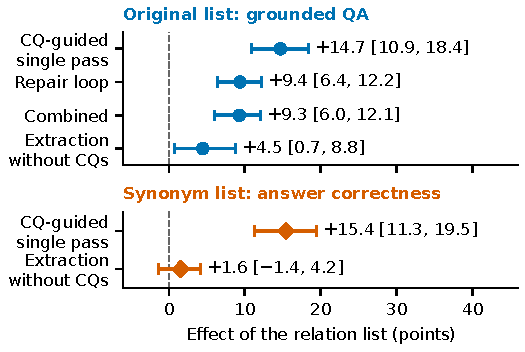
\includegraphics[width=\columnwidth]{figures/fig_seed_forest.pdf}
\caption{The relation list raised held-out grounded QA in all four pipelines, and synonym names raised answer correctness in the CQ-guided single pass. Differences in points with 95\% intervals, Qwen on 2Wiki; the groups use different metrics, so compare within a group only.}
\label{fig:seedforest}
\end{figure}


\paragraph{Synonym and outside-shard lists also help.}
A synonym list sharing no word stem with the original raised the CQ-guided single pass's answer correctness by 15.4 points (Figure~\ref{fig:seedforest}, Appendix~\ref{app:synseed}), and a list induced from passages outside the T-REx evaluation shards raised its grounded QA by 7.4 points (Appendix~\ref{app:trexlist}).



\section{One List-Guided Pass Against Costlier Pipelines}
\label{sec:res-cost}

\paragraph{Seeded extraction costs a fraction of the loop's tokens.}
At one seventh to one seventeenth of the tokens, seeded extraction is above the repair loop on HotpotQA and on T-REx with the 2Wiki list; on the original 2Wiki shards and on T-REx with its own induced list the two are indistinguishable (the loop's 2Wiki gains are in Section~\ref{sec:res-loop}). Table~\ref{tab:glance} gives the contrasts. The loop used 6.7 to 8.3 times the tokens of seeded extraction on 2Wiki, 7.1 on HotpotQA and 16 to 17 on T-REx.

\paragraph{The list-schema pass leads the combined pipeline and the repair loop.}
Paired on all 60 main-run units, it is 4.6 points above the combined pipeline and 5.3 above the repair loop, at about one eighth of the combined pipeline's tokens (106k against 838k per unit). The combined pipeline's first pass alone already scores .607 at 277k tokens (Table~\ref{tab:exp8}), so the lead does not come from the extra passes. It is also 4.9 points above seeded extraction in grounded QA and level with it in answer correctness; Table~\ref{tab:glance} lists these contrasts and the answer-correctness margins. The lead over the combined pipeline holds with an embedding retriever (+4.2 grounded QA) and with BM25 plus dense fusion (+4.5), and over the repair loop as well (Appendix Table~\ref{tab:altret}).

\paragraph{With an induced list the list-schema pass still scores above the combined pipeline.}
An induced list comes from the corpus alone, not from gold relations. With the same induced list given to both, on 60 units, the list-schema pass scores .616 grounded QA against .563 for the combined pipeline (+5.3 [2.0, 9.0]; answer correctness +1.5 [$-$1.9, 4.8]) at 104k tokens per unit against 769k. It is 2.5 points above the repair loop ([$-$0.2, 5.2]; 806k tokens) and 3.4 above seeded extraction (Table~\ref{tab:glance}).

\paragraph{Reference point: HippoRAG 2.} HippoRAG 2~\cite{gutierrez2025hipporag2} answers from its top-5 passages, while our arms answer from graph facts. On the same 2Wiki chunks, with the same Qwen builder and answerer, seeded extraction scored .678 answer correctness against .671 for HippoRAG 2 (+0.7, interval spanning 0). It used half the tokens: 128k against 268k per unit, counting queries (the 106k figure elsewhere counts construction only; Appendix~\ref{app:external}).

\paragraph{Reference point: LightRAG.} On the same chunks and with the same answerer, LightRAG~\cite{guo2024lightrag} (mix mode, library defaults) answers from about 13k tokens of entities, relations and passages per question. On the same 30 shards it scored .721 answer correctness. The list-schema pass, answering from 60 graph facts, was level with it ($-$3.2 [$-$7.5, 0.7]) at one seventh of its tokens (124k against 909k per unit, counting queries); seeded extraction trailed it by 4.3 ([$-$8.1, $-$0.1]) and the combined pipeline by 6.6 ([$-$10.5, $-$2.9]).

\begin{figure*}[t]
\centering
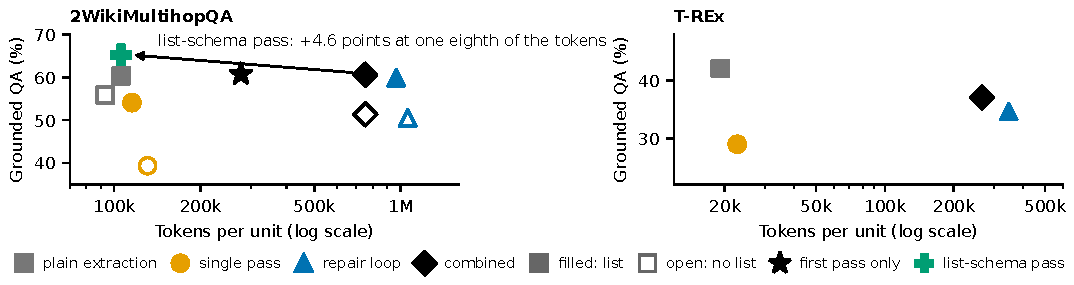
\includegraphics[width=0.9\textwidth]{figures/fig_cost_quality.pdf}
\caption{The list-schema pass (green) scored 4.6 points above the combined pipeline in grounded QA at one eighth of its construction tokens, and seeded extraction matched the combined pipeline at the same low cost. Arm means against tokens per unit (log axis; overlapping points shifted sideways slightly); intervals are in Table~\ref{tab:glance} and Appendix Tables~\ref{tab:glanceall} and~\ref{tab:itext}. Left, 2Wiki (60 units). Right, T-REx, arms with the list only. Qwen.}
\label{fig:costquality}
\end{figure*}


\paragraph{Reference point: three public extractors.}
Each public extractor ran with its released settings, and its graph facts were scored with our retriever and answerer on the same chunks. Plain extraction scored .558 grounded QA on the 60 main-run units (30 shards $\times$ 2 runs); iText2KG scored 12.8 points lower and EDC 11.4 (4 to 6 points lower with an embedding retriever), and AutoSchemaKG's entity-relation triples 34.6 lower on the 30 units it ran (Appendix~\ref{app:external}, Table~\ref{tab:itext}). Given the 22 names as its pre-defined target schema, EDC scored 14.6 points below seeded extraction on the same 30 units.




\section{Where the Repair Loop Wins: Bridge-Comparison Questions and Small Fact Caps}
\label{sec:res-loop}

The repair loop wins on fresh 2Wiki shards, on bridge-comparison questions and at small answer fact caps, and loses on comparison questions, at large caps and on HotpotQA.

\paragraph{Pooled over 60 2Wiki shards, the loop leads seeded extraction by 3.2 points.}
Over the 30 original and 30 fresh shards the loop leads by 3.2 points in grounded QA ([0.2, 6.5]), almost all of it on bridge-comparison questions, and the two are level in answer correctness (Table~\ref{tab:glance}). Guided repair did not beat random patches of the same size (+1.9 [$-$1.6, 5.3]; Appendix Table~\ref{tab:glanceall}).

\paragraph{On the original 2Wiki shards the two are level, with opposite signs by question type.}
A bridge-comparison question compares an attribute of two entities, each reached through a bridge entity (for example, which of two films has the older director). With the list, the repair loop (.599 grounded QA at 878k tokens per unit) and seeded extraction (.603 at 106k) were level (Tables~\ref{tab:glance} and~\ref{tab:exp8}); seeded extraction holds more facts (1,472 against 980 per unit), and the loop trails it by 4.0 points in answer correctness and 4.9 in relation accuracy (Appendix Table~\ref{tab:glanceall}). By question type, on these original shards, the loop led by 22.5 points on bridge-comparison questions and trailed by 14.2 on comparison questions (Appendix Table~\ref{tab:qtype}).

\paragraph{Fresh shards favor the repair loop on 2Wiki and seeded extraction on HotpotQA.}
On fresh shards (question shards no earlier run used) the loop was 6.9 points ahead of seeded extraction in grounded QA on 2Wiki and 18.2 behind on HotpotQA.

\paragraph{Under hybrid QA the loop's lead shrinks as the fact cap loosens.}
Under hybrid QA (graph facts plus passages: the answerer sees 30 graph facts and the top 3 passages), the loop's answer correctness exceeds seeded extraction's .585 by 8.5 points ([5.5, 11.8]; 2Wiki, 60 units = 30 shards $\times$ 2 runs; Appendix Table~\ref{tab:newchecks}). Seeded extraction scores lower here than graph-only at 60 facts (.678): the 30-fact cap binds for 70\% of its questions (see the cap sweep below). With up to 60 graph facts plus the same passages, seeded extraction trails the loop by only 1.6 points ($-$1.6 [$-$4.4, 0.8]; .709 against .725, 30 shards).

\paragraph{With the same induced list, the loop keeps its bridge-comparison lead.}
With the same induced list in both arms (the outside-shard list, 30 shards), the two were level in grounded QA overall but the bridge-comparison lead remained (18.3 points with the induced list; 120 questions), and on T-REx a T-REx-induced list closed the gap (Appendix Table~\ref{tab:glanceall}).

\paragraph{Small fact caps favor the loop, large ones seeded extraction.}
The answer fact cap is the number of facts the answerer sees (default 60; Figure~\ref{fig:capsweep}, Appendix~\ref{app:factcap}). On 2Wiki (60 units) the loop leads at caps of 10 to 30 and seeded extraction at 120; on HotpotQA (30 units) seeded extraction leads at every cap. Re-answered the same way on 2Wiki, the list-schema pass is above the repair loop at every cap and above the combined pipeline up to 60 facts; at 120, where no cap binds and its answerer sees 26 facts per question against 44, the two are level (Appendix~\ref{app:factcap}).




\begin{figure}[t]
\centering
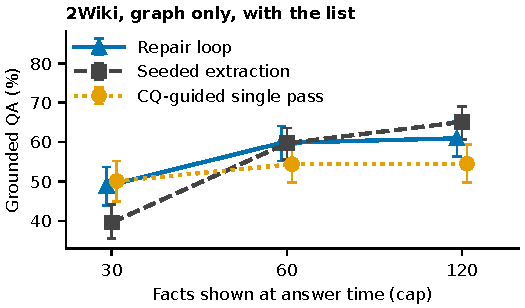
\includegraphics[width=0.88\columnwidth]{figures/fig_capsweep.pdf}
\caption{Grounded QA on 2WikiMultihopQA when the answer step sees only the first 30, 60 or 120 retrieved facts from the stored graphs (60 units; bars are 95\% intervals over 30 shard clusters).}
\label{fig:capsweep}
\end{figure}

\begin{table}[!tb]
\centering
\caption{Arm means on 2WikiMultihopQA (Qwen); Table~\ref{tab:arms} defines the arms. ``Combined, first pass only'' is the combined pipeline stopped after its first extraction pass. QA is held-out grounded QA and Rec. is uncapped evidence recall (capped recall: Appendix~\ref{app:heldout}). Facts and tokens (Tok.) are per shard and run, tokens in thousands. Tokens of ``Combined, no list'' (a dash) match the combined pipeline's budget. Paired contrasts are in Table~\ref{tab:glance}.}
\label{tab:exp8}
\footnotesize\setlength{\tabcolsep}{2.5pt}
\begin{tabular}{lcccc}
\toprule
 & QA & Rec. & Facts & Tok. (k) \\
\midrule
Single pass & .394 & .646 & 725 & 131 \\
Single pass, with list & .541 & .761 & 687 & 108 \\
Repair loop & .505 & .768 & 1,134 & 1,061 \\
Repair loop, with list & .599 & .845 & 980 & 878 \\
Plain extraction & .558 & .874 & 1,704 & 100 \\
Seeded extraction & .603 & .895 & 1,472 & 106 \\
Combined & .606 & .901 & 1,435 & 838 \\
Combined, no list & .514 & .798 & 1,418 & --- \\
Combined, first pass only & .607 & .854 & 972 & 277 \\
List-schema pass & .652 & .873 & 742 & 106 \\
\bottomrule
\end{tabular}
\end{table}

\begin{table*}[t]
\centering
\caption{Loop against seeded extraction, and the list-schema pass against four arms (Qwen): grounded QA in points unless marked, first arm minus second arm as written in each row, 95\% intervals; ``loop'' is the repair loop, ``seeded'' seeded extraction, ``list-schema'' the list-schema pass; ``Same'' repeats the row above for answer correctness; both-with-list rows build both arms with the induced list; $n$ is the number of shards; 60 units = 30 shards $\times$ 2 runs, pooled shards = 30 original + 30 fresh. T-REx graphs use the 2Wiki list. Arms: Table~\ref{tab:arms}; other contrasts: Appendix Tables~\ref{tab:glanceall} and~\ref{tab:itext}.}
\label{tab:glance}
\footnotesize\setlength{\tabcolsep}{2pt}
\begin{tabular}{P{5.6cm}P{5.0cm}P{3.0cm}P{3.3cm}}
\toprule
 Contrast & 2Wiki & T-REx (orig. $n$=33) & HotpotQA (orig. $n$=30) \\
\midrule
Loop $-$ seeded, original shards & $-$0.4 [$-$3.6, 2.8] ($n$=30) & $-$7.5 [$-$11.7, $-$3.8] & $-$15.2 [$-$18.8, $-$11.7] \\
Loop $-$ seeded, fresh shards & +6.9 [2.1, 11.7] (.631 against .563; $n$=30 fresh) & & $-$18.2 [$-$25.5, $-$6.3] (.292 against .474; $n$=12 fresh) \\
Loop $-$ seeded, 60 shards pooled & +3.2 [0.2, 6.5] ($n$=60 shards) & & \\
Same, answer correctness & $-$0.3 [$-$3.2, 2.4] (original $-$4.0 [$-$7.7, $-$0.7], fresh +3.3 [$-$1.0, 7.3]) & & \\
Bridge-comparison, 60 shards pooled, loop $-$ seeded & +23.3 [16.9, 30.0] ($n$=60 shards) & & Bridge $-$15.1 [$-$18.9, $-$10.6] ($n$=42 shards) \\
Comparison, 60 shards pooled, same & $-$10.8 [$-$16.9, $-$5.4] ($n$=60 shards) & & $-$20.8 [$-$31.4, $-$12.3] ($n$=42 shards) \\
List-schema $-$ combined, 60 units & Grounded QA +4.6 [1.3, 7.8]; answer correctness +3.3 [$-$0.1, 6.0] & & \\
List-schema $-$ loop, 60 units & Grounded QA +5.3 [2.2, 8.4]; answer correctness +5.0 [2.4, 7.4] & & \\
List-schema $-$ seeded, 60 units & Grounded QA +4.9 [1.0, 9.4]; answer correctness +1.0 [$-$2.6, 4.3] & & \\
Induced list: list-schema $-$ combined, 60 units & Grounded QA +5.3 [2.0, 9.0]; answer correctness +1.5 [$-$1.9, 4.8] & & \\
Induced list: list-schema $-$ loop, 60 units & Grounded QA +2.5 [$-$0.2, 5.2]; answer correctness +2.1 [$-$0.8, 4.6] & & \\
Induced list: list-schema $-$ seeded, 60 units & Grounded QA +3.4 [0.4, 6.9]; answer correctness +0.4 [$-$2.9, 4.1] & & \\
List-schema, induced $-$ original list, 30 units & Grounded QA $-$2.7 [$-$6.9, 1.0] & & \\
Tokens per unit, loop vs seeded & 878k against 106k (original); 699k against 105k (fresh) & 310k against 19.1k & 942k against 133k \\
\bottomrule
\end{tabular}
\end{table*}



\section{SPARQL: the List Gives Queryable Predicates}
\label{sec:res-cqs}

On held-out 2Wiki questions, a compact schema fixed by the relation list gives the whole SPARQL advantage over seeded extraction. The test uses questions nobody generated: the 16 held-out evaluation questions per shard that grounded QA also uses, with the gold answer as the expected span (30 units). The list-schema pass passes 34.9\% of them, level with the combined pipeline (34.9\%) and 27.4 points above seeded extraction (7.5\%), which receives the same list in its prompt (Table~\ref{tab:sparql}). It holds about half the combined pipeline's facts at one eighth of its tokens.

\begin{table}[t]
\centering
\caption{SPARQL pass rate on held-out 2Wiki questions (Qwen, 30 units), differences in points with 95\% intervals. Renamed: the model mapped each seeded predicate to a list name or kept it; list-named only keeps the mapped triples. Arms: Table~\ref{tab:arms}.}
\label{tab:sparql}
\footnotesize\setlength{\tabcolsep}{3pt}
\begin{tabular}{@{}p{2.45cm}c>{\raggedright\arraybackslash}p{4.75cm}@{}}
\toprule
Arm & Pass (\%) & Difference, points [95\% CI] \\
\midrule
List-schema pass & 34.9 & \\
Combined pipeline & 34.9 & Combined $-$ list-schema +0.0 [$-$3.7, 3.4] \\
Seeded extraction & 7.5 & List-schema $-$ seeded +27.4 [22.8, 31.9] \\
Extraction, no list & 13.4 & List-schema $-$ this row +21.5 [17.8, 25.6] \\
Seeded, renamed & 21.8 & List-schema $-$ this row +13.1 [9.1, 16.9] \\
Seeded, list-named only & 32.4 & List-schema $-$ this row +2.6 [$-$1.6, 6.4] \\
List-schema, induced & 28.3 & List-schema $-$ seeded, both induced +16.1 [12.8, 19.4] \\
Seeded, induced & 12.2 & List-schema, induced $-$ original list $-$6.6 [$-$10.3, $-$3.5] \\
List-named, induced & 21.0 & List-schema, induced $-$ this row +7.4 [4.7, 11.0] \\
CQ-guided single pass & 32.1 & Single pass $-$ list-schema $-$2.8 [$-$7.4, 1.3] \\
Repair loop & 31.5 & \\
\bottomrule
\end{tabular}
\end{table}

\paragraph{Three scorers.}
Table~\ref{tab:sparql} uses the Qwen judge on 30 units (one run seed); the scorer comparison here pools 54 units from two run seeds. Scorers: a rule (the gold answer is in the returned rows), a Qwen judge and a second LLM judge from another model family, Claude Haiku 5.5. Over these 54 units, the combined pipeline minus the list-schema pass is +3.5 [0.8, 6.1] under the rule, +0.0 [$-$2.7, 2.6] under the Qwen judge and $-$2.1 [$-$4.4, 0.7] under the Haiku judge, so it has no edge under either judge and leads only under the rule.

\paragraph{The gap is the vocabulary the facts are stored under.}
Mapping each predicate to one of the 22 list names, or leaving it, mapped 48.3\% of the triples and raised the pass rate from 7.5\% to 21.8\% (+14.3 [11.2, 17.4]); about 339 properties remained. Shown each graph's 22 most frequent predicates, the query writer lifts seeded extraction to 22.1\%, still 19.0 points [14.9, 23.3] below the list-schema pass given the same summary (41.0\%). Cut to the list-named triples only (712 facts), seeded extraction comes level with the list-schema pass (32.4\%, +2.6 [$-$1.6, 6.4]); with an induced list it stays 7.4 points [4.7, 11.0] behind (Table~\ref{tab:sparql}; Appendix~\ref{app:sparqlchecks}). The advantage over seeded extraction does not depend on the hand-written list: with an induced list the list-schema pass still passes 28.3\% against 12.2\% for seeded extraction (+16.1 [12.8, 19.4]).

\paragraph{The combined pipeline answers its own generator's questions better.}
On fresh CQs written by the pipeline's generator (Appendix~\ref{app:freshcq}), the combined pipeline leads the list-schema pass by 18.1 points ([15.4, 21.4]), the measure CQs are built for; on held-out questions it shows no edge.

\section{Discussion}
\label{sec:discussion}

\paragraph{What to use.}
\begin{enumerate}[nosep,label=(\roman*)]
  \item For SPARQL or other querying over a closed relation vocabulary on 2Wiki-like corpora with a small relation inventory, where a gold or induced list exists, use the list-schema pass: it scores 4.6 points above the combined pipeline in grounded QA and is level with it in SPARQL pass rate under the Qwen judge, at about one eighth of its tokens (Sections~\ref{sec:res-cost} and~\ref{sec:res-cqs}).
  \item To answer from graph facts on corpora with many long-tail relations (HotpotQA-like), build plain extraction with and without the list, twice one build's tokens, and compare them on a validation split, since the effect depends on the corpus and the list (+4.5 on 2Wiki with the original list, +0.8 with an induced one, +0.5 on T-REx, $-$4.0 on HotpotQA). Choosing on a validation half of the shards was reliable for effects of about 4 points or more (Appendix~\ref{app:heldout}).
  \item On 2Wiki-like corpora the repair loop leads seeded extraction on bridge-comparison questions, at 7 to 8 times the tokens; use it there only if that cost is acceptable. On HotpotQA-like corpora seeded extraction leads at every fact cap.
\end{enumerate}

\paragraph{Limitations.}
The list-schema pass's advantage holds for small relation inventories; on HotpotQA it is 20.4 points below seeded extraction. The findings rest on one builder family, Qwen, with Gemma replicating some studies in the appendix (Appendix~\ref{app:addedvalues} and~\ref{app:loopfurther}). The corpora are Wikipedia-derived with short chunks; T-REx is a 14-relation one-hop movie subset and HotpotQA is one run. The 2Wiki list is derived from the training split's gold evidence; induced lists use no gold. The list is a flat relation vocabulary: typed schemas, entity resolution and graph updates were not studied.

\section{Conclusion}
\label{sec:conclusion}

In our rebuilt CQ pipeline family on 2Wiki, the held-out QA gain comes from the relation list: one extraction pass given only the list is level with the combined pipeline in answer correctness at about one eighth of its tokens and leads it in grounded QA when the answerer sees up to 60 facts, with a corpus-induced or a gold-derived list. Chunk-generated CQs and the repair loop multiply the cost; the loop leads seeded extraction on bridge-comparison questions, on fresh shards and at small fact caps, and trails it on comparison questions and on HotpotQA. A compact list also makes the graph queryable: SPARQL over the list-schema graph passes 34.9\% of held-out tests against 7.5\% for seeded extraction, and guided repair did not beat random patches of equal size. On long-tailed inventories such as HotpotQA the list can hurt, so compare builds with and without it on your own validation questions.


\bibliographystyle{IEEEtran}
\bibliography{references}

\appendices
\renewcommand{\arraystretch}{0.85}\setlength{\textfloatsep}{6pt plus 2pt minus 2pt}\setlength{\dbltextfloatsep}{6pt plus 2pt minus 2pt}\setlength{\floatsep}{6pt plus 1pt minus 1pt}\setlength{\dblfloatsep}{6pt plus 1pt minus 1pt}
\section{Additional Results and Records}
\label{app:experiments}

The main study is the 2Wiki study of Table~\ref{tab:exp8}. KG-only QA is grounded QA's graph-only setting.

\begin{table*}[!t]
\centering
\caption{Results of the contrasts of Tables~\ref{tab:glance} and~\ref{tab:listeffect} on the original shards, and of the remaining contrasts in the study. Values are differences in points unless marked; $n$ is the number of shards; where two run seeds were used, 30 shards $\times$ 2 run seeds = 60 units. Result reads the interval: improved when the 95\% interval excludes 0 on the higher side, lower when it lies below 0, not established when it includes 0. A dash means no interval is listed in the row.}
\label{tab:glanceall}
\scriptsize\setlength{\tabcolsep}{2pt}
\begin{tabular}{P{3.5cm}P{9.4cm}P{0.8cm}P{3.9cm}}
\toprule
Claim & Experiment, model and corpus; contrast; value [95\% interval] & $n$ & Result \\
\midrule
The list raises grounded QA & Main, Qwen, 2Wiki. Values in Table~\ref{tab:listeffect}. & 30 & --- \\
Synonym list, answer correctness & Main, Qwen, 2Wiki. Synonym list $-$ no list. L0 +15.4 [11.3, 19.5]; U-ext +1.6 [$-$1.4, 4.2]. & 30 & improved (L0); not established (U-ext) \\
Induced list raises answer correctness & Main, Qwen, 2Wiki; T-REx. Values in Table~\ref{tab:listeffect}. & 30; 33 & improved \\
Outside-shard list raises grounded QA & Main, Qwen, T-REx. L0, list induced outside the evaluation shards $-$ no list: +7.4 [3.9, 11.4]. & 33 & improved \\
Graph above chunk retrieval & Main, Qwen, 2Wiki. Seeded extraction $-$ retrieval of top 5 chunks; with list hint. +15.4 [10.6, 19.8]; +16.9 [11.1, 22.3]; no-context answer model .325 [.294, .354]. & 30 & improved \\
Equal fact count: guided pass above selections & Main, Qwen, 2Wiki. Guided pass $-$ selections of the extraction graph at the guided pass's fact count ; values in Table~\ref{tab:selection}. & 30 & with list, no selection above the guided pass; without list, relation frequency above \\
List-schema pass above CQ-guided pass & Qwen, 2Wiki; T-REx. Values in Table~\ref{tab:listschema}. & 30; 33 & improved \\
Expansion, grounded QA & First and second patch, Qwen, 2Wiki. G $-$ L0. +9.1 [4.7, 13.8]; +9.6 [5.2, 14.8]. & 40; 24 & improved \\
Iteration vs.\ one batch of CQs & Iteration, Qwen, 2Wiki. Iteration $-$ one batch, recall. +1.2 [$-$3.5, 5.7], crossed shard $\times$ run seed interval. & 24 & not established \\
Hybrid QA with 160 vs.\ 40 CQs & CQ-count, as above. 160 vs.\ 40 CQs, 1$\times$. $-$3.6 to +0.6, all intervals include 0 (Table~\ref{tab:exp9}). At 4$\times$ budget, Qwen 2Wiki $-$9.1 [$-$13.8, $-$5.5]. & 20--33 & not established at 1$\times$; lower at 4$\times$ \\
Guided repair vs.\ random & First and second patch, Qwen, 2Wiki. Guided $-$ random patches, grounded QA: +1.9 [$-$1.6, 5.3] ($n$=40); $-$0.3, one-sided upper bound 3.1 ($n$=24). & 40; 24 & first patch study: not established; second: upper bound below margin 5 \\
Loop against seeded extraction & Main, Qwen, 2Wiki; T-REx. Values in Table~\ref{tab:glance}. & 30; 33 & --- \\
Loop $-$ seeded extraction, induced list, grounded QA & Qwen, 2Wiki. Outside-shard induced list in both arms. +2.3 [$-$1.0, 6.0]; bridge-comparison +18.3 [7.5, 29.2], comparison $-$10.0 [$-$18.3, $-$4.2]; T-REx list $-$1.1 [$-$5.6, 2.4] (17.0$\times$ the tokens). & 30; 33 & not established; bridge-comparison improved, comparison lower; T-REx not established \\
Loop with list $-$ seeded extraction at the loop's fact count, grounded QA & Main, Qwen, 2Wiki; seeded graphs cut at random to the loop's fact count (three draws; 60 units). Loop $-$ cut seeded +31.6 [27.1, 35.9] (answer correctness +25.2 [21.0, 29.8]); full graphs $-$0.9 [$-$4.4, 2.1] ($-$4.7 [$-$8.2, $-$1.7]); full seeded $-$ cut seeded +32.5 [28.8, 36.5]. & 30 & improved (loop $-$ cut seeded); not established (full graphs) \\
Loop with list $-$ seeded extraction, entity-pair coverage and relation correctness & Main, Qwen, 2Wiki, scored by code. Entity-pair coverage $-$5.8 [$-$7.3, $-$4.1] (comparison $-$15.0 [$-$19.8, $-$10.2]; bridge-comparison 0.0 [$-$1.3, 1.5]); relation correctness within matched pairs +0.4 [$-$1.1, 1.5]; relation accuracy $-$4.9 [$-$6.7, $-$2.8]. & 30 & lower (entity-pair coverage, relation accuracy); not established (relation correctness) \\
Seeded extraction against HippoRAG 2, answer correctness & Main chunks, Qwen, 2Wiki. Against HippoRAG 2 (top 5 passages; chain-of-thought answerer): seeded extraction +0.7 [$-$4.0, 5.2]; +1.4 [$-$2.0, 4.1]. Loop with list $-$3.2 [$-$7.4, 1.1]; $-$2.5 [$-$5.2, 0.2]. Combined $-$1.6 [$-$5.9, 2.4]; +1.1 [$-$2.0, 4.2]. & 30 & not established \\
Loop $-$ seeded extraction, induced list, answer correctness & As above. $-$0.4 [$-$3.5, 2.5]; T-REx list $-$2.9 [$-$7.6, 0.6]. & 30; 33 & not established \\
Seeded extraction, induced $-$ training-split list, grounded QA & As above. $-$3.5 [$-$7.7, $-$0.2]; the loop, +0.2 [$-$2.7, 3.1]. & 30 & lower (seeded extraction); not established (loop) \\
HotpotQA arms & Added corpus, Qwen, HotpotQA, grounded QA. Seeded extraction .488 (2,231 facts and 646 relation names, 133k tokens; plain extraction 2,435 facts and 964 names), loop .335 (1,268 facts, 942k), U-ext .527; L0 with the induced list .281, without .192; list-schema pass .283; U-ext $-$ seeded extraction +4.0 [0.2, 8.1]. Other contrasts are in Section~\ref{sec:res-schema} and Table~\ref{tab:glance}. & 30 & Seeded extraction vs loop: seeded non-inferior and above (loop minus seeded $-$15.2; margin 5; 0.0008). List vs no list: improved (0.0004). List-schema vs L0 with list: not established. U-ext vs seeded: improved \\
Combined vs.\ loop, recall & Main, Qwen, 2Wiki. Combined $-$ LOOP+vocab, recall. Uncapped +5.6 [4.2, 7.0]; capped $-$8.7 [$-$10.6, $-$6.8]; equal fact counts +1.1 [0.5, 1.9]. & 30 & improved (uncapped); lower (capped); improved (equal fact counts) \\
Seeded extraction vs.\ combined & Main, Qwen, 2Wiki. Seeded extraction $-$ Combined, QA. $-$0.3 [$-$3.9, 2.8]; 106k per unit against 277k (first pass) and 838k (full run); answer correctness +2.3 [$-$0.2, 4.4]; T-REx, grounded QA, seeded extraction $-$ combined +5.0 [0.4, 8.6], 19.1k against 298k. & 30 & not established; T-REx improved \\
Combined passes more fresh CQs & Main, Qwen, 2Wiki. Combined $-$ seeded extraction +13.5 [10.7, 16.2] (60 units, original scoring; +12.3 [9.8, 14.9] with the judge rerun); combined $-$ plain extraction +1.3 [$-$1.2, 3.9] by judge (rerun), +6.3 [3.6, 8.9] by rule (60 units); Claude Haiku 5.5 judge in Appendix~\ref{app:freshcq}; held-out-question rows in Table~\ref{tab:listschema}. & 30 & improved (vs.\ seeded extraction); not established (vs.\ plain extraction, judge); improved (rule) \\
\bottomrule
\end{tabular}
\end{table*}

\begin{table*}[t]
\centering
\caption{Three public extractors against the arms of Table~\ref{tab:exp8} (Qwen, 2Wiki), in two blocks with different units. EDC ran with its released settings (Self Canonicalization). The EDC row with and without the list is on the 30 units. AutoSchemaKG's entity-relation triples are the comparable variant; its full graph also holds concept and event edges. Tokens are per unit, in thousands. Differences are the extractor minus the arm, in points, with 95\% intervals.}
\label{tab:itext}
\scriptsize\setlength{\tabcolsep}{3pt}
\begin{tabular}{lcccc}
\toprule
 & Grounded QA & Answer correctness & Facts & Tokens (k) \\
\midrule
\multicolumn{5}{l}{\emph{60 units (30 shards, two run seeds)}} \\
iText2KG & .430 [.393, .470] & .549 [.503, .596] & 1,899 & 478.8 \\
EDC & .445 [.398, .493] & .629 [.583, .676] & 1,358 & 618.4 \\
Plain extraction (U-ext) & .558 & .648 & 1,704 & 100.0 \\
Seeded extraction & .603 & .678 & 1,472 & 105.9 \\
Combined & .606 & .655 & 1,435 & 837.7 \\
Single pass (L0) & .394 & .433 & 725 & 131.0 \\
iText2KG $-$ U-ext & $-$12.8 [$-$16.5, $-$8.6] & $-$9.9 [$-$13.3, $-$5.8] & & \\
EDC $-$ U-ext & $-$11.4 [$-$15.2, $-$7.5] & $-$1.9 [$-$5.2, 1.8] & & \\
iText2KG $-$ seeded extraction & $-$17.3 [$-$21.0, $-$13.9] & $-$12.9 [$-$16.3, $-$10.0] & & \\
iText2KG $-$ combined & $-$17.6 [$-$20.8, $-$14.1] & $-$10.6 [$-$14.1, $-$7.5] & & \\
iText2KG $-$ single pass & $+$3.6 [$-$1.5, 9.3] & $+$11.6 [5.6, 18.2] & & \\
EDC $-$ seeded extraction & $-$15.8 [$-$19.3, $-$12.3] & $-$4.9 [$-$7.7, $-$2.5] & & \\
EDC $-$ combined & $-$16.1 [$-$20.1, $-$12.4] & $-$2.6 [$-$5.9, 0.5] & & \\
EDC $-$ single pass & $+$5.1 [0.5, 10.0] & $+$19.6 [14.8, 24.7] & & \\
\midrule
\multicolumn{5}{l}{\emph{30 units (30 shards, one run seed)}} \\
EDC, 22-name list / no list & .458 / .454 & .613 / .633 & 824 / 1,356 & 791 / --- \\
AutoSchemaKG, entity-relation triples & .213 [.175, .252] & .446 [.396, .490] & 1,257 & 1,557.8 \\
AutoSchemaKG, full graph & .096 [.073, .121] & .233 [.200, .260] & 18,360 & 1,557.8 \\
AutoSchemaKG triples $-$ U-ext & $-$34.6 [$-$38.5, $-$30.8] & $-$20.2 [$-$23.8, $-$16.7] & & \\
AutoSchemaKG triples $-$ seeded extraction & $-$39.2 [$-$44.0, $-$34.4] & $-$23.3 [$-$27.5, $-$20.0] & & \\
AutoSchemaKG triples $-$ combined & $-$41.9 [$-$46.3, $-$38.3] & $-$23.1 [$-$27.3, $-$19.0] & & \\
AutoSchemaKG triples $-$ single pass & $-$19.2 [$-$26.0, $-$13.1] & $+$2.1 [$-$5.0, 9.4] & & \\
\bottomrule
\end{tabular}
\end{table*}


\begin{table*}[!ht]
\centering
\caption{CQ-count study, other arms against the reference of 40 CQs at 1$\times$, in points. The arms with 160 CQs have shard-cluster BCa 95\% intervals; the 40-CQ arm at 4$\times$ is an arm-mean difference with no interval. Tokens are the mean ratio of 160 CQs at 4$\times$ to the reference.}
\label{tab:exp9other}
\scriptsize\setlength{\tabcolsep}{2.5pt}
\begin{tabular}{p{4.1cm}cccc}
\toprule
 & Qwen, T-REx & Gemma, T-REx & Gemma, 2Wiki & Qwen, 2Wiki \\
\midrule
KG-only QA, 160 CQs, 4$\times$ & +4.7 [1.6, 8.0] & +5.0 [1.7, 8.2] & +10.6 [2.5, 17.2] & +1.6 [$-$4.7, 5.7] \\
KG-only QA, 40 CQs, 4$\times$ (mean) & +1.5 & $-$0.5 & +1.0 & 0.0 \\
Evidence recall, 160 CQs, 4$\times$ & +1.9 [0.8, 3.9] & +0.6 [$-$0.2, 2.0] & +9.5 [5.9, 15.6] & +12.0 [8.8, 15.6] \\
Hybrid QA, 160 CQs, 4$\times$ & +0.9 [$-$2.8, 4.2] & +0.3 [$-$2.1, 2.6] & $-$0.9 [$-$4.7, 3.4] & $-$9.1 [$-$13.8, $-$5.5] \\
Precision, 160 CQs, 4$\times$ & $-$12.4 [$-$18.0, $-$7.8] & $-$1.2 [$-$4.8, 2.4] & +3.3 [$-$0.6, 7.1] & $-$12.2 [$-$17.0, $-$6.4] \\
Precision, 160 CQs, 1$\times$ & 0.0 [$-$5.2, 5.0] & $-$0.5 [$-$5.2, 3.8] & +4.9 [0.8, 9.4] & $-$4.0 [$-$9.0, 0.7] \\
Tokens, 160 CQs 4$\times$ / reference & 2.8 & 1.9 & 3.8 & 4.0 \\
\bottomrule
\end{tabular}
\end{table*}

\begin{table*}[!t]
\centering
\caption{CQ-count study: 160 CQs at the 1$\times$ token budget against the reference of 40 CQs at 1$\times$. Differences in points with shard-cluster BCa 95\% intervals; $n$ is the number of shards in the contrast. 90\% intervals for hybrid QA, left to right: [$-$1.8, 2.3], [$-$1.7, 3.1], [$-$3.4, 4.7] and [$-$8.1, 0.3].}
\label{tab:exp9}
\footnotesize\setlength{\tabcolsep}{3.5pt}
\begin{tabular}{lcccc}
\toprule
 & Qwen, T-REx & Gemma, T-REx & Gemma, 2Wiki & Qwen, 2Wiki \\
 & ($n$=33) & ($n$=26) & ($n$=20) & ($n$=24) \\
\midrule
Hybrid QA & +0.3 [$-$2.2, 2.6] & +0.6 [$-$2.2, 3.6] & +0.6 [$-$3.7, 5.6] & $-$3.6 [$-$8.9, 1.0] \\
KG-only QA & +3.5 [0.7, 6.8] & +5.6 [2.0, 9.8] & +10.9 [4.1, 15.9] & +6.2 [0.3, 10.4] \\
Evidence recall (uncapped) & +0.3 [$-$1.1, 2.1] & +1.0 [0.1, 2.3] & +9.2 [5.5, 15.4] & +9.9 [6.9, 13.2] \\
\bottomrule
\end{tabular}
\end{table*}

\begin{table*}[!ht]
\centering
\caption{Original Qwen runs and the Gemma replication, in points with 95\% intervals ($n$ in shards or units). For the second patch study the margin is 5 points. A dash means no value or no run. The building-ontology study contrasts iterative CQ refinement with none, not with extraction. Nemotron is a third model whose grounded QA stayed at floor (at most .047 in every arm).}
\label{tab:replication}
\scriptsize\setlength{\tabcolsep}{3pt}
\begin{tabular}{P{4.6cm}P{3.9cm}P{4.7cm}P{3.9cm}}
\toprule
Experiment and contrast & Qwen & Gemma & Nemotron \\
\midrule
Building-ontology, iteration over none (by construction, plan) & +21.4 [16.2, 27.1] & +42.1 [33.6, 50.7] & invalid or at floor \\
First patch, GR over L0 & +9.7 [4.1, 15.0] & +13.1 [7.8, 18.4] & invalid or at floor \\
Second patch, evaluation-guided over random repair & $-$0.3, upper bound 3.1 (one-sided), not improved & +1.5 [$-$3.1, 6.5], not improved & $-$0.7 [$-$1.9, 0.0] \\
Main, recall, combined over LOOP+vocab & +5.6 [4.2, 7.0] & +9.2 [7.6, 11.4] ($n$=60) & +13.1 [8.9, 16.8] ($n$=41) \\
Main, recall, combined over L0+vocab & +14.0 [12.1, 15.9] & +10.2 [2.1, 16.1] & +16.7 [11.8, 20.9] \\
Main design on T-REx, combined $-$ LOOP+vocab & --- & +1.6 [$-$0.9, 4.4], not established ($n$=27) & +1.2 [$-$0.6, 4.1], not established ($n$=12) \\
Main design on T-REx, combined $-$ L0+vocab & --- & +2.7 [$-$0.4, 5.8], not established & --- \\
\bottomrule
\end{tabular}
\end{table*}

\begin{table*}[!ht]
\centering
\caption{Checks added after the main study, Qwen. Hybrid QA answer correctness with up to 30 or 60 graph facts (60: a rerun; a dash: not tabulated), the 30-fact column against vector-only QA (.502 [.460, .544]) and fact precision judged by Gemma, both on the 2Wiki main-study graphs (points, 95\% intervals, 30 shards, 60 units); grounded QA, class-aligned recall and tokens per unit (thousands) for the main-study arms on T-REx (33 shards, one run seed).}
\label{tab:newchecks}
\scriptsize\setlength{\tabcolsep}{2.5pt}
\begin{tabular}{lccccccc}
\toprule
 & Hybrid QA, 30 facts & Hybrid QA, 60 facts & Hybrid $-$ vector & Precision & Grounded QA, T-REx & Recall, T-REx & Tokens (k) \\
\midrule
L0 & .600 & --- & +9.8 [4.3, 14.6] & --- & --- & --- & --- \\
L0+vocab & .692 & .716 & +19.0 [14.7, 22.5] & .874 [.856, .890] & .290 & .173 & 22.7 \\
LOOP+vocab & .671 & .725 & +16.9 [12.2, 21.0] & .802 [.785, .819] & .346 & .189 & 310 \\
Combined & .603 & .699 & +10.1 [5.3, 14.2] & .716 [.686, .741] & .371 & .228 & 298 \\
U-ext+vocab & .585 & .709 & +8.3 [2.2, 13.9] & .925 [.913, .938] & .421 & .184 & 19.1 \\
\bottomrule
\end{tabular}
\end{table*}

\begin{table*}[!ht]
\centering
\caption{List-schema runs and the Gemma structured-query run (Qwen builds the graphs; $n$ shard $\times$ run seed units). Arm values for the first and second arm: grounded QA and facts per unit; in the fresh-CQ and held-out-question rows, pass rates (30-unit rows: the run seed with all graphs). Differences in points, shard-cluster BCa 95\% intervals. Arm values differ between rows because the contrasts come from separate runs (the first row's .529 is the list-schema study's own run of the single pass given the list, .541 in Table~\ref{tab:exp8}).}
\label{tab:listschema}
\scriptsize\setlength{\tabcolsep}{3pt}
\begin{tabular}{P{7.8cm}P{2.0cm}P{4.2cm}P{3.0cm}}
\toprule
Contrast & Corpus, $n$ & Arm values & Difference \\
\midrule
List-schema pass $-$ CQ-guided single pass & 2Wiki, 30 & .650, 734 facts; .529, 657 & +12.1 [7.5, 16.0] \\
List-schema pass $-$ CQ-guided single pass & T-REx, 33 & .335, 111 facts; .291, 109 & +4.4 [1.0, 7.4] \\
List-schema pass $-$ CQ-guided single pass & HotpotQA, 30 & .283, 1,339 facts; .281, 927 & +0.2 [$-$5.0, 4.8] \\
List-schema prompt with 40 CQs $-$ CQ-guided single pass & 2Wiki, 30 & .617, 810 facts; .529, 649 & +8.8 [4.8, 12.9] \\
List-schema pass (separate run) $-$ list-schema prompt with 40 CQs & 2Wiki, 30 & .644, 756 facts; .617, 810 & +2.7 [$-$0.2, 5.6] \\
Factorial run: CQ-derived schema cut to 22 properties $-$ CQ-guided single pass & 2Wiki, 30 & .537, 610 facts; .535, 684 & +0.2 [$-$1.9, 2.9] \\
Factorial run: CQ-derived schema restricted to the 22 names $-$ CQ-guided single pass & 2Wiki, 30 & .608, 681 facts; .535, 684 & +7.3 [3.3, 12.1] \\
Factorial run: list-schema pass $-$ CQ-derived schema restricted to the 22 names & 2Wiki, 30 & .650, 734 facts; .608, 681 & +4.2 [0.6, 7.3] \\
Combined $-$ seeded extraction, fresh-CQ pass rate, Qwen judge, original scoring & 2Wiki, 60 & .410; .275 & +13.5 [10.7, 16.2] \\
Same, Gemma writes and judges & 2Wiki, 60 & .369; .231 & +13.8 [11.6, 16.2] \\
Same, Qwen writing and judging rerun on the stored graphs (rerun scoring) & 2Wiki, 60 & --- & +12.3 [9.8, 14.9] \\
Same, rescored without a judge (rows $\le$ 20, expected span in result) & 2Wiki, 60 & .479; .314 & +16.5 [13.9, 19.0] \\
Combined $-$ list-schema pass, fresh-CQ pass rate & 2Wiki, 30 & .414; .233 & +18.1 [15.4, 21.4] \\
Combined $-$ plain extraction, fresh-CQ pass rate & 2Wiki, 30 & .414; .381 & +3.3 [$-$0.7, 7.1] \\
Loop given the list; single pass given the list, fresh-CQ pass rate (arm means only) & 2Wiki, 30 & .375; .330 & --- \\
Combined $-$ plain extraction, rescored without a judge & 2Wiki, 60 & .479; .416 & +6.3 [3.6, 8.9] \\
Held-out questions: combined $-$ seeded extraction & 2Wiki, 60 & .348; .074 & +27.3 [23.4, 31.1] \\
Same, combined $-$ plain extraction & 2Wiki, 60 & .348; .131 & +21.7 [18.0, 25.7] \\
Same, combined $-$ its first pass & 2Wiki, 60 & .348; .316 & +3.2 [2.0, 4.2] \\
Same, combined first pass $-$ seeded extraction & 2Wiki, 60 & .316; .074 & +24.1 [20.1, 27.8] \\
Same, combined $-$ list-schema pass (judge; rule only) & 2Wiki, 30 & .349; .349 (rule .402; .377) & +0.0 [$-$3.7, 3.4]; +2.5 [$-$0.8, 5.7] \\
Same, list-schema pass $-$ seeded extraction; $-$ plain extraction & 2Wiki, 30 & .349; .075; .134 & +27.4 [22.8, 31.9]; +21.5 [17.8, 25.6] \\
Same, CQ-guided single pass $-$ list-schema pass & 2Wiki, 30 & .321; .349 & $-$2.8 [$-$7.4, 1.3] \\
Same, second set (other run seed, separate list-schema run): combined $-$ list-schema pass (judge; rule only) & 2Wiki, 24 & .331; .326 (rule .406; .349) & +0.4 [$-$2.6, 3.7]; +5.7 [2.3, 8.9] \\
Same, rule only, combined $-$ seeded extraction; $-$ plain extraction & 2Wiki, 60 & .409; .116; .204 & +29.3 [25.8, 32.8]; +20.5 [16.9, 24.8] \\
Seeded extraction $-$ plain extraction, fresh-CQ pass rate & 2Wiki, 30 & .275; .381 & $-$10.7 [$-$13.6, $-$7.8] \\
Same, 60 units, rerun scoring & 2Wiki, 60 & --- & $-$11.1 [$-$13.3, $-$8.7] \\
\bottomrule
\end{tabular}
\end{table*}

\begingroup\footnotesize
\subsection{Further relation-list checks}
\label{app:seednames}
\paragraph{Relation list names.} Table~\ref{tab:seednames} lists the 22 names of each 2Wiki list, copied from the list files, in alphabetical order.

\begin{table}[t]
\centering
\caption{The original list (relation names taken from the 2WikiMultihopQA training split), the induced list (proposed by an LLM from 300 corpus chunks), and a list induced the same way from 300 chunks outside the evaluation shards.}
\label{tab:seednames}
\scriptsize\setlength{\tabcolsep}{3pt}
\begin{tabular}{lP{6.6cm}}
\toprule
Original & award received, cause of death, child, composer, country, country of citizenship, country of origin, date of birth, date of death, director, educated at, father, founded by, inception, mother, occupation, performer, place of birth, place of burial, place of death, publication date, spouse \\
Induced & award, based on, birth date, birth place, cast member, child, country, death date, death place, director, employer, genre, located in, member of, nationality, occupation, parent, position held, release year, sibling, spouse, title \\
Induced outside shards & based on, birth date, birth place, cast member, child, death date, death place, director, employer, genre, location, member of, nationality, occupation, parent, producer, publication date, release year, sibling, spouse, title, writer \\
\bottomrule
\end{tabular}
\end{table}

\paragraph{Synonyms and alignment.}
In U-ext the synonym list's answer correctness was $-$1.5 points against the original list ([$-$4.2, 1.4]). A re-analysis of stored predictions tests the original list's gain without name matching (Table~\ref{tab:seedalign}). For the three pipelines that use CQs the effect stays above zero on both measures, and class-free recall keeps 65 to 85\% of the class-aligned effect.

\begin{table}[!htb]
\centering
\caption{List effect in points (95\% BCa intervals, 30 shards, 60 units), main study. Class-free recall ignores relation classes when matching triples to gold; answer correctness drops the grounding requirement.}
\label{tab:seedalign}
\scriptsize\setlength{\tabcolsep}{2.5pt}
\begin{tabular}{lccc}
\toprule
 & Recall, class aligned & Class-free recall & Answer correct \\
\midrule
L0 & +11.4 [9.3, 14.5] & +9.7 [7.6, 12.9] & +13.8 [10.5, 17.2] \\
LOOP & +7.7 [5.4, 9.7] & +5.0 [2.9, 6.9] & +7.9 [4.8, 10.7] \\
Combined & +10.3 [8.0, 12.6] & +6.8 [5.1, 8.6] & +7.0 [4.0, 9.7] \\
U-ext & +2.1 [1.0, 3.5] & +0.6 [$-$0.7, 2.3] & +3.0 [0.0, 6.6] \\
\bottomrule
\end{tabular}
\end{table}

\subsection{Seeded extraction against the combined pipeline}
A 90\% interval of [$-$3.3, 2.3] around the difference in grounded QA, seeded minus combined (Section~\ref{sec:res-cost}) excludes differences beyond about 3 points. On T-REx the combined pipeline found more gold evidence (class-aligned recall +4.4, 90\% [3.0, 6.0]).

\subsection{Fact-count check and coverage}
With the list, U-ext raised grounded QA over L0+vocab by 6.3 points ([2.6, 9.4]).


\begin{table}[!htb]
\centering
\caption{Guided single pass minus a selection of the extraction graph at the guided pass's fact count (Qwen on 2Wiki, 60 shard $\times$ run seed units; grounded QA, differences in points with 95\% intervals). Result states which pass scores higher. The selectors read no questions or gold relations; one arm reads the unit's CQs; the random subset is a uniform draw. Selectors keep: most frequent relations; most central entities; most connected two-hop paths (chain); facts the answer model rates most informative from the chunk (model); BM25 match to the 40 CQs (CQ); round-robin by chunk (balanced).}
\label{tab:selection}
\scriptsize\setlength{\tabcolsep}{3pt}
\begin{tabular}{llcl}
\toprule
Selection & Relation list & Guided $-$ selection & Result \\
\midrule
Entity centrality & none & +14.4 [9.3, 19.3] & guided higher \\
Relation frequency & none & $-$8.0 [$-$13.5, $-$3.0] & selection higher \\
Entity centrality & seeded & +25.8 [20.3, 30.3] & guided higher \\
Relation frequency & seeded & +16.6 [11.2, 21.9] & guided higher \\
Chain-preserving & seeded & +25.0 [19.8, 30.1] & guided higher \\
Model-scored & seeded & +14.3 [8.9, 19.3] & guided higher \\
CQ-selected & seeded & +33.3 [28.3, 37.7] & guided higher \\
Chunk-balanced & seeded & +37.2 [31.6, 41.4] & guided higher \\
Random subset & none & +28.2 [23.2, 33.0] & guided higher \\
Random subset & seeded & +39.1 [34.0, 43.9] & guided higher \\
\bottomrule
\end{tabular}
\end{table}

\subsection{Hybrid QA and CQ count}
\label{sec:res-hybrid}
Tables~\ref{tab:exp9other} and~\ref{tab:exp9} give the results at each CQ count. On the main-study graphs (Qwen, 2Wiki), hybrid QA scored above vector-only QA (.502 [.460, .544]) in every pipeline (Table~\ref{tab:newchecks}). In the CQ-count study, four times as many CQs at the same budget raised KG-only QA in all four settings (Table~\ref{tab:exp9}); hybrid QA did not separate from the 40-CQ reference.



\subsection{Answer-time fact cap}
\label{app:factcap}
The stored graphs were answered again at caps of 10 to 120 facts with the same retrieval, prompt, answerer and scorer (Qwen); cap $k$ keeps the first $k$ facts of the cap-120 retrieval, and the cap-60 rerun matched the stored retrieval on every question. On 2Wiki, seeded extraction $-$ loop was $-$9.3 ([$-$13.2, $-$5.7]) at 30 facts and +4.2 ([1.2, 7.2]) at 120; on HotpotQA seeded extraction led by 5.6 at 10 facts and 17.7 at 120. The list-schema pass minus the combined pipeline was +9.8 to +11.7 at caps of 10 to 30, +3.4 [0.2, 6.4] at 60 in this rerun (+4.6 in the main run) and $-$0.4 [$-$3.2, 2.4] at 120; minus the repair loop it was +4.1 to +5.8 at every cap.


\paragraph{Reach intervention.}\label{app:reach}
On the stored 2Wiki graphs (6 arms $\times$ 60 units), adding the held gold-evidence facts to the 60 the answerer saw raised answer correctness by 4.3 to 10.0 points and removing them lowered it by 40.4 to 62.5 (Holm $p \le .0007$).


\paragraph{Alternative retrievers.}\label{app:altret}
The stored graphs were answered with the 60 nearest facts under Qwen3-Embedding-0.6B (no entity linking or hop expansion) or with its rank fusion with our retriever (2Wiki, 8 arms $\times$ 60 units; HotpotQA, 5 arms $\times$ 30 units). Grounded QA on 2Wiki was 10 to 24 points lower under the embedding retriever; Table~\ref{tab:altret} gives the contrasts. Under BM25+dense the combined pipeline fell behind seeded extraction ($-$2.6 [$-$4.5, $-$0.5]).

\begin{table}[t]
\centering
\caption{Contrasts in grounded QA (points, 95\% intervals) under our retriever and two alternative answer-time retrievers (Qwen, stored graphs). 2Wiki rows use 60 units and the HotpotQA row 30. Last row: list effect on plain extraction. List-schema grounded QA .427 (embedding), .415 (fusion). Intervals are BCa, so a reversed contrast is not the mirror image of its interval elsewhere.}
\label{tab:altret}
\scriptsize\setlength{\tabcolsep}{1.5pt}
\begin{tabular}{P{2.35cm}P{2.1cm}P{2.1cm}P{2.1cm}}
\toprule
Contrast & Ours (BM25) & Embedding & BM25+dense \\
\midrule
Loop+list $-$ seeded & $-$0.4 [$-$3.6, 2.8] & $-$2.5 [$-$5.3, 0.4] & $-$4.0 [$-$6.6, $-$1.2] \\
List on single pass & +14.7 [10.9, 18.4] & +6.5 [3.5, 9.2] & +5.6 [2.6, 8.6] \\
EDC $-$ plain extraction & $-$11.4 [$-$15.2, $-$7.5] & $-$6.2 [$-$9.4, $-$3.0] & $-$7.4 [$-$10.4, $-$4.3] \\
iText2KG $-$ plain extraction & $-$12.8 [$-$16.5, $-$8.6] & $-$4.0 [$-$7.3, $-$0.6] & $-$6.8 [$-$10.4, $-$3.9] \\
HotpotQA loop $-$ seeded & $-$15.2 [$-$18.8, $-$11.7] & $-$14.4 [$-$17.9, $-$11.2] & $-$14.8 [$-$19.4, $-$11.5] \\
List-schema $-$ combined & +4.6 [1.3, 7.8] & +4.2 [0.8, 7.2] & +4.5 [1.1, 7.7] \\
Combined $-$ seeded & +0.3 [$-$3.0, 3.6] & $-$0.2 [$-$2.4, 1.9] & $-$2.6 [$-$4.5, $-$0.5] \\
List effect & +4.5 [0.7, 8.8] & +2.3 [$-$0.4, 4.9] & +2.3 [0.1, 4.6] \\
\midrule
List-schema $-$ loop & --- & +6.5 [2.8, 9.9] & +5.8 [2.2, 9.4] \\
List-schema $-$ seeded & --- & +4.0 [1.1, 6.7] & +1.9 [$-$1.6, 5.3] \\
\bottomrule
\end{tabular}
\end{table}

\subsection{Question types and operations}
\begin{table}[t]
\centering
\caption{Grounded QA contrasts on 2Wiki by question type (points, 95\% intervals; Qwen, 30 shards, 4 questions per type per shard) and by number of gold evidence items. Evidence count and type overlap: the three-or-more group is 120 bridge-comparison and 7 comparison questions.}
\label{tab:qtype}
\scriptsize\setlength{\tabcolsep}{1.5pt}
\begin{tabular}{P{2.45cm}P{2.2cm}P{2.2cm}P{2.2cm}}
\toprule
Type ($n$ questions) & Loop+list $-$ seeded & Single pass+list $-$ single pass & Combined $-$ seeded \\
\midrule
Comparison (120) & $-$14.2 [$-$21.7, $-$7.5] & +13.3 [6.3, 19.6] & $-$0.8 [$-$6.7, 4.6] \\
Bridge-comparison (120) & +22.5 [14.2, 31.7] & +28.8 [18.8, 38.3] & +8.3 [$-$1.7, 17.5] \\
Compositional (120) & $-$5.0 [$-$11.3, 0.4] & +10.0 [3.8, 16.7] & 0.0 [$-$7.1, 5.8] \\
Inference (120) & $-$5.0 [$-$12.9, 2.5] & +6.7 [0.8, 11.7] & $-$6.3 [$-$12.9, 0.8] \\
All (480) & $-$0.4 [$-$3.6, 2.8] & +14.7 [10.9, 18.4] & +0.3 [$-$3.0, 3.6] \\
\midrule
2 evidence items (353) & $-$7.8 [$-$11.3, $-$4.4] & +9.4 [5.6, 13.2] & $-$1.9 [$-$5.0, 1.4] \\
$\ge$3 evidence items (127) & +21.3 [13.0, 30.7] & +28.9 [19.4, 39.0] & +7.9 [$-$0.8, 17.5] \\
\bottomrule
\end{tabular}
\end{table}
Per unit, the loop and the combined pipeline took a median of 2,000 s and 1,935 s against 103 s for seeded extraction (about 19 times; concurrency differed); the Gemma loop with the list failed in 7 of 60 units from output cut or invalid JSON after retries.

\subsection{Combined pipeline versus the loop}
Without a per-question triple cap the combined pipeline led in all three models (Table~\ref{tab:replication}), and at equal fact counts the lead shrank to +1.1 [0.5, 1.9] in Qwen, +0.3 [$-$0.6, 1.1] in Gemma and +0.3 [$-$0.5, 1.3] in Nemotron. In Qwen, capped recall favoured the loop (Tables~\ref{tab:exp8} and~\ref{tab:glanceall}).


\subsection{Further checks}
Of the 2,196 gold evidence facts in the iteration-study graphs, 860 were reproduced exactly, 74 had a wrong value, 96 were split across entities and 1,166 were missing. Omissions made up 87.3\% of the 1,336 inexact facts. SHACL shapes~\cite{knublauch2017shacl} flagged 0.15\% of the inexact facts ([0, 0.37]) and 25.1\% of correct facts.

\paragraph{Loop against seeded extraction, further checks.}\label{app:loopfurther} With Gemma on 2Wiki the loop differed from seeded extraction by $-$0.2 points [$-$4.5, 4.0] on the 53 of 60 units that completed and by $-$5.6 [$-$11.1, $-$0.6] when failed units count as 0, the rule of the replication analyses.


\paragraph{Held-out test of the list decision.}\label{app:heldout} Each pair of graphs with and without the list was split at random into halves, 1,000 times; a validation half held 15 to 17 shards (about 16 questions each). The validation half added the list when its mean grounded QA difference was above 0; the choice was right when the test half's value for it was at least that of the other side. Right choices: single pass 100\% on all three corpora; extraction 96.8\% on 2Wiki with the original list, 43.7\% with the induced list (mean difference +0.8), 25.6\% on T-REx and 96.0\% on HotpotQA. Test losses were at most 1.0 point.


\paragraph{Prompt-optimisation study.}\label{app:promptopt} On 400 test questions the fixed list reached evidence recall .425, against .363 for MIPROv2 and .356 for GEPA.

\subsection{CQ-count study arms and measures}
\label{app:exp8def}
The reference arm uses 40 CQs at the 1$\times$ token budget, which for each shard comes from a reference run; an arm stops after using 95\% of it. Other arms are named by CQ count and budget (160 CQs at 1$\times$ and 4$\times$, 40 CQs at 4$\times$). The source check regenerates a CQ up to 3 times when its embedding (Qwen3-Embedding-0.6B) does not match the top 5 retrieved chunks.

In the CQ-count study, KG-only QA gives the answerer graph facts only.

\begin{table*}[!t]
\centering
\scriptsize\setlength{\tabcolsep}{3pt}\renewcommand{\arraystretch}{0.7}
\caption{The eight studies (the error analysis varies no component, the others each vary one), and the Gemma replication.}
\label{tab:experiments}
\begin{tabular}{lp{9.4cm}p{5.0cm}l}
\toprule
Study & Question & Data & Models \\
\midrule
Building-ontology study & Does iterative CQ refinement improve a graph? & Building ontology bank, 35 test questions & Qwen \\
Iteration study & Does iteration improve on one batch of the same CQs? & 2Wiki, 24 shards & Qwen \\
Prompt-optimisation study & Does prompt optimisation improve on a relation list? & 2Wiki, 400 test questions & Qwen \\
First patch study & Does a CQ $\rightarrow$ SPARQL $\rightarrow$ judge $\rightarrow$ patch loop help? & 2Wiki, 40 shards & Qwen \\
Second patch study & Does a loop with query repair and a rejecting gate help? & 2Wiki, 24 shards $\times$ 2 run seeds & Qwen \\
Error analysis & Which error types occur, and can Shapes Constraint Language (SHACL) see them? & iteration-study graphs & --- \\
Main study & What do the combined pipeline's parts add? & 2Wiki, 30 shards $\times$ 2 run seeds & Qwen \\
CQ-count study & How do CQ count, budget and hybrid QA interact? & 2Wiki and T-REx, 20 to 33 shards & Qwen, Gemma \\
Replication & Gemma (building-ontology, patch and main studies; main design on T-REx) & as above & Gemma \\
\bottomrule
\end{tabular}
\end{table*}

\subsection{Scoring, token and selector details}
\label{app:details}
\paragraph{Further arms.}\label{app:armsextra} G is the CQ-guided single pass (L0) with CQs expanded to every chunk; GR adds evaluate-and-repair rounds to G; L0+vocab$K$ gives L0 $K$ of the 22 names ($K$ = 6, 11, 17; nested random subsets). All three use CQs and take the list where L0 does.

\paragraph{Metric definitions.}\label{app:metricdefs}
\begin{itemize}
  \item \emph{Evidence recall}: \emph{uncapped recall} counts every matching triple. \emph{Capped recall} is recall under a per-question triple budget $B$, so padding the graph lowers it; the formula, $B$ and the slice follow below.
  \item \emph{Relation accuracy} (the share of gold evidence triples with a fact on the right entity pair, relation and direction) is scored by code against the gold relation names (23 for 2Wiki, 14 for T-REx) and a synonym and inverse-relation table fixed in advance. \emph{Entity-pair coverage} is the share with a fact on the right entity pair under any relation, and \emph{relation correctness within matched pairs} the share of those pairs with the right relation and direction. HotpotQA's gold evidence names no relation, so the measure is undefined there.
  \item The \emph{pass rate of fresh CQs} uses 40 new CQs per shard and run, written from random chunks with a neutral prompt and no relation list. SPARQL is generated three times for each CQ from the graph's schema (its classes and a slice of the 15 properties whose names and types share the most word stems with the question, not its facts); a query passes when it returns the expected answer span and the judge scores it 2, and the pass rate is the mean over the three generations.
  \item \emph{Hybrid QA} gives the answerer graph facts and retrieved passages, and \emph{vector QA} gives it passages only. KG-only QA: Appendix~\ref{app:exp8def}.
\end{itemize}

\paragraph{Evidence recall.} A gold evidence triple counts as present when a chunk-cited triple links the same entity pair under a predicate of the same relation class. The capped-recall budget is two triples for every source sentence of the question's paragraphs, and the hypergeometric expectation is computed exactly. A question's graph slice is the set of triples extracted from the chunks of its own ten paragraphs. For gold evidence $e$ with $m_e$ matches among the $N$ triples of the slice and budget $b=\min(B,N)$, the evidence counts $1-\binom{N-m_e}{b}/\binom{N}{b}$; capped recall is the mean over gold evidence.

\paragraph{Answer correctness.} Normalised exact match against the gold answer and its aliases or demonyms, the first token for yes/no questions, exact match for dates; ``unknown'' counts as wrong.

\paragraph{External extractors and HippoRAG 2.}\label{app:external}
iText2KG 1.1.0 (no incremental merging), EDC~\cite{zhang2024edc} (Self Canonicalization) and AutoSchemaKG~\cite{bai2026autoschemakg} (triples; 30 shards, one run) ran once per chunk on the main study's 2Wiki chunks with Qwen and were scored by its answerer and scorer; only one EDC run took the 22 names (Appendix Table~\ref{tab:itext}). HippoRAG 2 used the same chunks, Qwen builder and answerer and Qwen3-Embedding-0.6B, answering from its top 5 passages, at 268k tokens per unit (204k construction, 64k queries; seeded extraction 128k on the same count).

\paragraph{Fresh-CQ pass rate by judge.}\label{app:freshcq}
The held-out-question rows of Table~\ref{tab:listschema} use the 16 evaluation questions of each shard in place of fresh CQs (gold answer as expected span, gold evidence chunks as the judge's source, three SPARQL generations). On the 30 units of run seed 20261101 the loop passed 31.5\% (arm values for the other arms in Table~\ref{tab:listschema}). A judge from another family (Claude Haiku 5.5) agreed with the Qwen judge on 91.9\% of final passes ($\kappa$ = .81).

\paragraph{Held-out SPARQL checks.}\label{app:sparqlchecks} On the 30 main-study 2Wiki units, a Claude Haiku 5.5 judge rescored the 4,718 regenerations that passed the rules, stricter than the Qwen judge, with the same ordering (list-schema pass minus seeded extraction +22.6 [19.4, 26.3]; combined minus list-schema pass $-$2.9 [$-$6.5, 0.3]).

\paragraph{Grounded QA definition.}\label{app:groundedqa} With $R(q, G) \subseteq G$ the facts retrieved for question $q$ from graph $G$, the indicator $\mathbb{I}_{\text{gc}}(q) \in \{0, 1\}$ is 1 when the answer generated from $R(q, G)$ is correct and grounded in those facts, and grounded QA over held-out questions $Q$ is $\frac{1}{|Q|}\sum_{q \in Q} \mathbb{I}_{\text{gc}}(q)$. The answerer sees graph facts and no passages (graph-only); retrieval and the grounding rule are in Appendix~\ref{app:groundedret}. QA-time retrieval is the same for every arm and does not use the list. The answerer sees at most 60 retrieved facts unless stated; Section~\ref{sec:res-loop} and Appendix~\ref{app:factcap} vary this cap.

\paragraph{Grounded QA retrieval.}\label{app:groundedret} For comparison questions every gold evidence pair (subject and object, in either direction) must appear in a retrieved fact that cites a chunk containing the evidence. For open questions the gold answer must appear as the subject or object of a retrieved fact. Relation classes enter only evidence recall (class-aligned recall). Also requiring the retrieved fact's relation class to match the gold relation lowers every arm by 0.7 to 2.9 points and leaves the gaps to the public extractors in place (seeded extraction minus iText2KG +18.8, against +17.3). The question is linked to entity labels (with aliases) by exact n-gram matching, the graph is followed for up to two hops, each entity contributes at most 25 facts ranked by BM25, and the facts in $R(q, G)$ are ordered by hop, then BM25, and capped at 60.


\paragraph{Fresh CQs, hybrid QA and precision.} Fact precision is judged on 40 sampled facts per graph; gold evidence covers only the facts that questions need, so unaligned triples are not counted as errors. Hybrid QA uses up to 30 graph facts (main run; a rerun used up to 60) and 3 passages, vector QA 5.

\paragraph{Decoding and tokens.} Cache hits count at full token cost. All models were served with vLLM, and Qwen ran with thinking off; six of the 60 main-run list-schema units were built later with the same weights on another engine instance. The QA answerer and extraction decode at temperature 0 (120 and 1,500 output tokens).

\subsection{Registration records and run details}
\label{app:registration}
\paragraph{List induction.}\label{app:induction}
The list is induced from the corpus being built, with no question and no gold relation: the extraction model reads 300 random passages (title and first 1,200 characters) in 20 batches of 15, proposes up to 15 relation names per batch, and one call merges the 80 names proposed in the most batches into exactly 22. A second 2Wiki list came the same way from 300 of 6,136 chunks outside the evaluation shards (5 of the 22 names of the original list, Jaccard .128); on T-REx the lists came from 300 of the 386 evaluation-corpus passages and from 96 passages outside the evaluation shards (Section~\ref{sec:res-schema}). On 2Wiki the induced list matched the gold relations for 62.2 (strict) to 72.0\% (lenient) of the evidence, the original list for 98.4\%. Inducing the 2Wiki list took 36,380 tokens and the T-REx list 75,691, once per corpus.

\paragraph{Statistics.}
Intervals are BCa bootstrap intervals over shards (B = 10,000); Holm correction is applied within each plan, and Table~\ref{tab:glanceall} gives each contrast's result.

\endgroup


\subsection{Supporting values by result}
\label{app:addedvalues}
\paragraph{List effects.}
In Gemma on 2Wiki the list raised grounded QA over no list by 7.4 points in the CQ-guided single pass ([3.3, 11.3]), 7.5 in the loop ([1.3, 15.0]) and 9.3 in the combined pipeline ([5.7, 12.9]). 



\subsection{Study overview and relation-list tables}
\label{app:movedtables}

\paragraph{T-REx lists.}\label{app:trexlist} Lists induced for T-REx (Qwen, 33 shards; outside-shard list one run seed), grounded QA and answer correctness: single pass, list $-$ none, +10.5 [6.0, 15.6] and +9.7 [5.5, 14.4]; plain extraction, list $-$ none, +0.5 [$-$2.5, 2.9] and +0.2 [$-$2.6, 2.7]; outside-shard list $-$ none, single pass, +7.4 [3.9, 11.4] and +6.8 [3.0, 10.9].

\paragraph{List content.}\label{app:seeddose} Answer correctness of the CQ-guided single pass by list content (2Wiki, 60 units; reruns): no list .417 [.366, .474], original list .568 [.521, .613], induced list .579 [.533, .620].

\paragraph{Synonym-list check.}\label{app:synseed} With 60 units (Qwen, 2Wiki), the synonym list minus no list was +15.4 [11.3, 19.5] in answer correctness and +12.4 [9.2, 16.0] in class-free recall (which ignores relation classes) for L0.



\end{document}
